\documentclass[tikz,border=10pt]{standalone}
\usepackage{tikz,amsmath}
\usetikzlibrary{arrows.meta,positioning,calc,fit,shapes.geometric}
\begin{document}
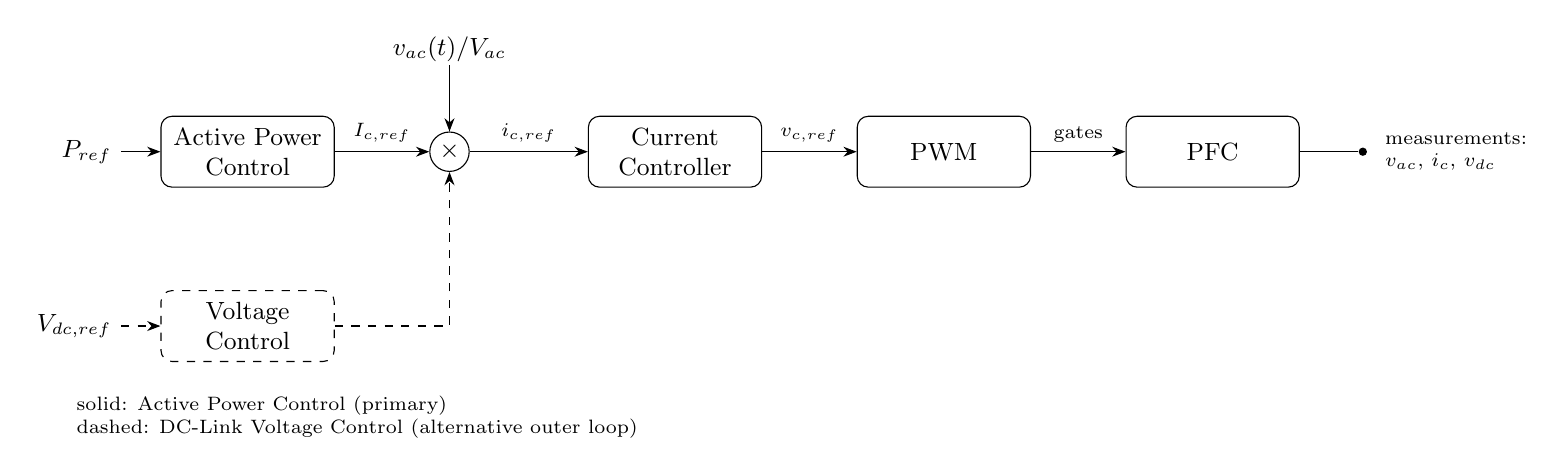
\begin{tikzpicture}[
  font=\small,
  >=Stealth,
  node distance=1.2cm,
  block/.style={draw, rounded corners, minimum width=2.2cm, minimum height=0.9cm, align=center},
  dashedblock/.style={draw, dashed, rounded corners, minimum width=2.2cm, minimum height=0.9cm, align=center},
  mul/.style={draw, circle, inner sep=0pt, minimum size=0.5cm},
  dot/.style={circle, fill=black, inner sep=0pt, minimum size=3pt},
]

% Primary path: P_ref -> Active Power Control -> multiply by v_ac/V_ac -> Current Controller -> PWM -> PFC
\node[block]        (PC)   at (0, 0)           {Active Power\\Control};
\node[mul, right=1.2cm of PC]  (M1)            {$\times$};
\node[block, right=1.5cm of M1]  (CC)          {Current\\Controller};
\node[block, right=1.2cm of CC]  (PWM)         {PWM};
\node[block, right=1.2cm of PWM] (PFC)         {PFC};

% Alternative path (dashed): V_dc,ref -> Voltage Control -> into multiplier (merges with primary route)
\node[dashedblock, below=1.3cm of PC]  (VC)    {Voltage\\Control};

% Input/output labels
\node[left=0.5cm of PC]   (Pref)  {$P_{ref}$};
\node[left=0.5cm of VC]   (Vref)  {$V_{dc,ref}$};

% v_ac/V_ac input to multiplier from above
\coordinate (vac_in) at ($(M1) + (0, 1.1)$);
\node at ($(vac_in) + (0, 0.2)$) {$v_{ac}(t)/V_{ac}$};

% Output from PFC
\node[right=0.6cm of PFC] (gates_out) {};
\coordinate (gates_right) at ($(PFC.east) + (1.8, 0)$);

% Wires (primary / solid)
\draw[->] (Pref)   -- (PC);
\draw[->] (PC)     -- node[above, font=\scriptsize]{$I_{c,ref}$} (M1);
\draw[->] (vac_in) -- (M1);
\draw[->] (M1)     -- node[above, font=\scriptsize]{$i_{c,ref}$} (CC);
\draw[->] (CC)     -- node[above, font=\scriptsize]{$v_{c,ref}$} (PWM);
\draw[->] (PWM)    -- node[above, font=\scriptsize]{gates} (PFC);

% Alternative path (dashed)
\draw[dashed, ->] (Vref)  -- (VC);
\draw[dashed, ->] (VC.east) -| (M1.south);

% Measurement feedback from PFC
\node[dot] (PFCout) at ($(PFC.east) + (0.8, 0)$) {};
\draw (PFC) -- (PFCout);

\coordinate (meas_bus) at ($(PFCout) + (0.6, 0)$);
\node[right=0.1cm of PFCout, align=left, font=\scriptsize] {measurements:\\$v_{ac},\, i_c,\, v_{dc}$};

% Legend
\node[font=\scriptsize, align=left] at ($(VC.south west) + (2.5, -0.7)$) {solid: Active Power Control (primary)\\dashed: DC-Link Voltage Control (alternative outer loop)};

\end{tikzpicture}
\end{document}
